\section{Sparse Optimization}

\begin{frame}{Two goals, one problem}
  \begin{tikzpicture}[remember picture,overlay]
    \draw [ultra thick,<->] ($(current page.north)+(-2.2,-0.32\textheight)$) -- ($(current page.north)+(2.2,-0.32\textheight)$) node (arrow) [midway] {};
    \node at ($(arrow.north)+(0,0.1)$) {\textbf{Sparse optimization}};
    \node [text width=0.3\textwidth] at ($(current page.north)+(-4,-0.3\textheight)$) (obs) {
        \begin{blockcolor}{Brown}{}
            \centering
            \textbf{Minimize a function}
        \end{blockcolor}
    };
    \node [text width=.3\textwidth] at ($(current page.north)+(4,-0.3\textheight)$) (dic) {
      \begin{blockcolor}{Brown}{}
            \centering
            \textbf{Sparse solution}
        \end{blockcolor}
    };
    %
    %
    %
    \node at ($(current page.north)+(-2.5,-0.65\textheight)$) (sp) {};
    \node at (sp) {Signal processing};
    \draw ($(sp)+(0,1)$) node {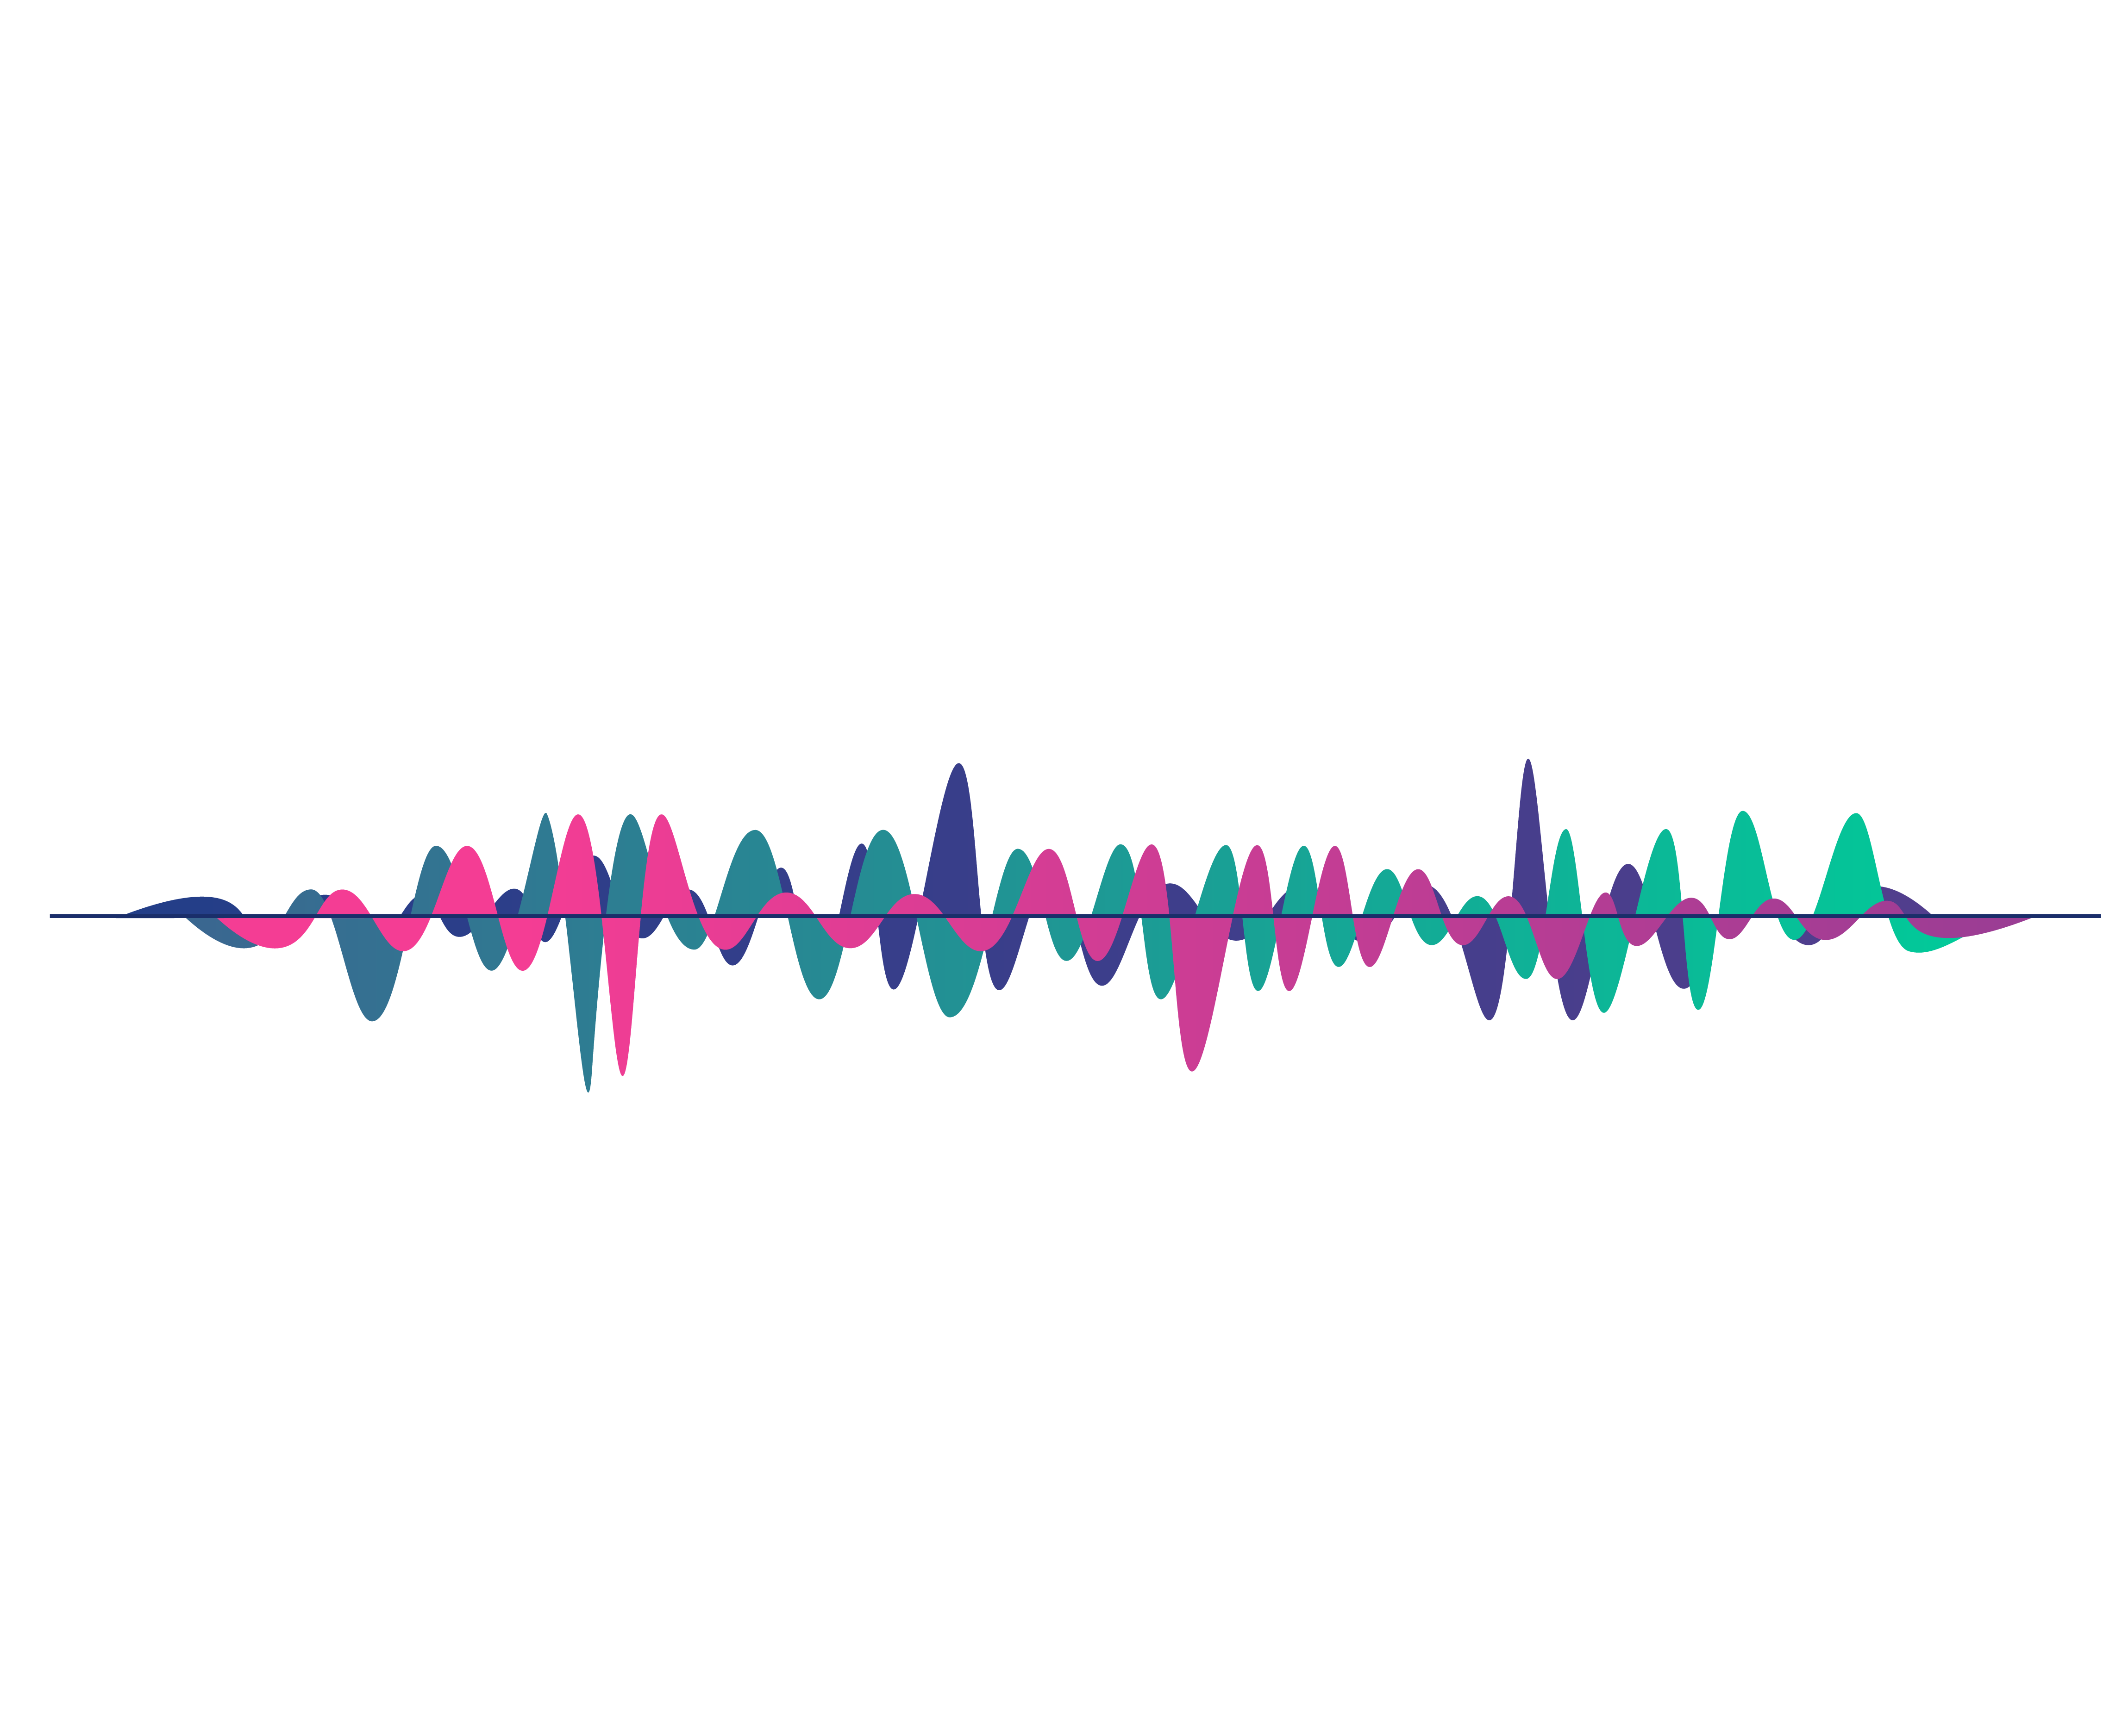
\includegraphics[width=4cm]{imgs/signal-processing.png}};
    %
    %
    %
    \node at ($(current page.north)+(2.5,-0.65\textheight)$) (ml) {};
    \node at (ml) {Machine learning};
    \draw ($(ml)+(0,1)$) node {
\includegraphics[width=2cm]{imgs/machine-learning.png}};
    %
    %
    %
    \node at ($(current page.north)+(-2.5,-0.95\textheight)$) (nd) {};
    \node at (nd) {Network design};
    \draw ($(nd)+(0,1.25)$) node {
\includegraphics[width=1.5cm]{imgs/network.png}};
    %
    %
    %
    \node at ($(current page.north)+(2.5,-0.95\textheight)$) (others) {};
    \node at (others) {And many others};
    \draw ($(others)+(0,1.25)$) node {
\includegraphics[width=1.25cm]{imgs/nerd_face.png}};
  \end{tikzpicture}
\end{frame}

\begin{frame}{Signal processing}
  \begin{tikzpicture}[remember picture,overlay]
    \onslide<+-> {
        \node at ($(current page.north)+(0,-0.2\textheight)$) {\textbf{Compressive sensing}};
        \node (center) at ($(current page.north)+(0,-0.5\textheight)$) {};
        %
        \node (groundtruth) at ($(center)+(-0.4\textwidth,0)$) {$\pv \in \kR^{\pdim}$};
        \node (groundtruth-text) at ($(groundtruth)+(0,0.05\textheight)$) {Sparse signal};
        \node (sensing) at ($(center)+(0,0.175\textheight)$) {Linear measurement through $\dic \in \kR^{\ddim\times\pdim}$};
        \node (observation) at ($(center)+(0.4\textwidth,0)$) {$\obs \in \kR^{\ddim}$};
        \node (observation-text) at ($(observation)+(0,0.05\textheight)$) {Observation};
        \node (recovery) at ($(center)+(0,-0.1\textheight)$) {\emphcolor{Brown}{Recover $\pv$ from $(\dic,\obs)$}};
        \draw [ultra thick,->] ($(groundtruth-text.north east)+(0,0)$) .. controls ($(sensing.south)+(0,0)$) .. ($(observation-text.north west)+(0,0)$);
        \draw [ultra thick,->] ($(observation-text.south west)+(0,0)$) .. controls ($(recovery.north)+(0,0)$) .. ($(groundtruth-text.south east)+(0,0)$);
        %
        %
        %
        \draw ($(groundtruth)+(0,-1)$) node {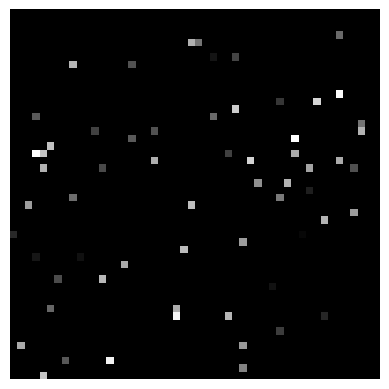
\includegraphics[width=1.5cm]{imgs/cs-x.png}};
        \draw ($(observation)+(0,-1)$) node {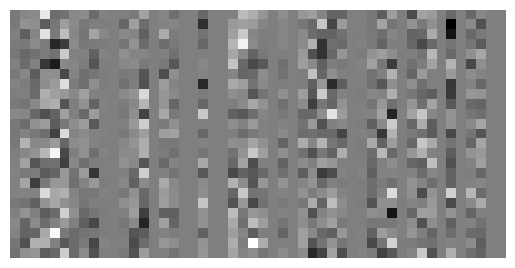
\includegraphics[width=2cm]{imgs/cs-y.png}};
        %
        %
        %
        \node [text width=0.5\textwidth] at ($(center)+(0,-0.3\textheight)$) (problem) {
            \begin{blockcolor}{black}{}
                \centering
                \textbf{Find $\pv$ such that $\obs \simeq \dic\pv$}
            \end{blockcolor}
        };
    }
    %
    %
    %
    \onslide<+-> {
        \node at ($(center)+(0,-0.39\textheight)$) (dimension) {$\ddim \ll \pdim$ : no unique solution};
    }
    %
    %
    %
    \onslide<+-> {
        \node [text width=0.5\textwidth] at ($(center)+(0,-0.3\textheight)$) (problem) {
            \begin{blockcolor}{black}{}
                \centering
                \textbf{Find $\pv$ \emphcolor{Brown}{sparse} such that $\obs \simeq \dic\pv$}
            \end{blockcolor}
        };
    }
  \end{tikzpicture}
\end{frame}

\begin{frame}{Machine learning}
    \begin{tikzpicture}[remember picture,overlay]
        \onslide<+-> {
            \node at ($(current page.north)+(0,-0.35\textheight)$) {
                \begin{tabular}{cccccc}
                    \multicolumn{6}{c}{\textbf{Heart disease dataset (LIBSVM)}} \\
                    \toprule
                    Age & Sex & Cholesterol & Blood pressure & ... & \textbf{Disease} \\
                    \midrule
                    31 & M & 50.3 mg/dl  & 95 mm/hg & ... & \textbf{No} \\
                    35 & F & 54.9 mg/dl & 98 mm/hg & ... & \textbf{Yes} \\
                    42 & F & 49.8 mg/dl & 92 mm/hg & ... & \textbf{Yes} \\
                    37 & M & 59.1 mg/dl & 89 mm/hg & ... & \textbf{No} \\
                    ... & ... & ... & ... & ... & ... \\
                    \bottomrule
                \end{tabular}
            };
        }
        %
        %
        %
        \onslide<+-> {
            \node[align=center,text width=0.2\textwidth] (data) at ($(current page.north)+(-4.5,-0.7\textheight)$) {
                \begin{blockcolor}{black}{}
                    \centering\textbf{Data}
                \end{blockcolor}
            };
            %
            \node[align=center,text width=0.3\textwidth] (logreg) at ($(current page.north)+(0,-0.7\textheight)$) {
                \begin{blockcolor}{black}{Logistic regression}
                    \centering$\min_{\pv} \ \text{LogLoss}(\pv)$
                \end{blockcolor}
            };
            \draw[ultra thick,->] ($(data.east)+(0.1,-0.2)$) -- ($(logreg.west)+(-0.1,-0.2)$);
            %
            \node[align=center,text width=0.2\textwidth] (estimator) at ($(current page.north)+(4.5,-0.7\textheight)$) {
                \begin{blockcolor}{black}{}
                    \centering\textbf{Estimator}
                \end{blockcolor}
            };
            \draw[ultra thick,->] ($(logreg.east)+(0.1,-0.2)$) -- ($(estimator.west)+(-0.1,-0.2)$);
        }
        %
        %
        %
        \onslide<+-> {
            \draw[ultra thick,<-,Brown] ($(estimator.south)+(-0.75,-0)$) .. controls ($(estimator.south)+(-1,-0.5)$) .. ($(estimator.south)+(-1,-1)$) node[below,align=center,text width=0.6\textwidth] {Involves all the features \\ Explainability and robustness issues};
        }
        %
        %
        %
        \onslide<+-> {
            \draw[ultra thick,<-,Brown] ($(logreg.south)+(-1.75,-0)$) .. controls ($(logreg.south)+(-2,-0.5)$) .. ($(logreg.south)+(-2,-1)$) node[below,align=center,text width=0.6\textwidth] {Force the use of only few \\ features via sparsity in $\pv$};
        }
    \end{tikzpicture}
\end{frame}

\begin{frame}{Finance}
    \begin{tikzpicture}[remember picture,overlay]
        \node[align=center,text width=0.45\textwidth] (problem) at ($(current page.north)+(0,-0.4\textheight)$) {
            \begin{blockcolor}{black}{Portfolio selection problem}
                \centering$\left\{\begin{array}{rl}
                    \max & \transp{\mathbf{c}}\pv - \tfrac{\sigma}{2}\transp{\pv}\Sigma\pv \\
                    \text{s.t.} & \transp{1}\pv = 1 \\
                    & \emphcolor{Brown}{\pv \ \text{is k-sparse}}
                \end{array}\right.$
            \end{blockcolor}
        };
        %
        \node[align=center,text width=0.7\textwidth] (xi) at ($(problem)+(1,-0.3\textheight)$) {\begin{itemize}
            \item[$\pvi{\idxentry}$ :] proportion of investment in asset i
            \item[$c_{\idxentry}$ :] profit of asset i
            \item[$\Sigma_{i,j}$ :] covariance of assets i and j
            \item[$k$ :] diversification budget
        \end{itemize}};
    \end{tikzpicture}
\end{frame}

\begin{frame}{Objective, constraint or both ?}
    \begin{tikzpicture}[remember picture,overlay]
        \onslide<+-> {
            \draw [ultra thick,<->] ($(current page.north)+(-2.2,-0.32\textheight)$) -- ($(current page.north)+(2.2,-0.32\textheight)$) node (arrow) [midway] {};
            \node at ($(arrow.north)+(0,0.1)$) {\textbf{Sparse optimization}};
            \node [text width=0.3\textwidth] at ($(current page.north)+(-4,-0.3\textheight)$) (obs) {
                \begin{blockcolor}{Brown}{}
                    \centering
                    \textbf{Minimize a function}
                \end{blockcolor}
            };
            \node at ($(current page.north)+(-4,-0.4\textheight)$) {\emphcolor{Brown}{Loss $\lossfunc(\pv)$}};
            \node [text width=.3\textwidth] at ($(current page.north)+(4,-0.3\textheight)$) {
            \begin{blockcolor}{Brown}{}
                    \centering
                    \textbf{Sparse solution}
                \end{blockcolor}
            };
            \node at ($(current page.north)+(4,-0.4\textheight)$) {\emphcolor{Brown}{Counting function $\norm{\pv}{0}$}};
        }
        %
        %
        %
        \onslide<+-> {
            \node [text width=0.4\textwidth] at ($(current page.north)+(-3,-0.6\textheight)$) (problem-constraint) {
                \begin{blockcolor}{black}{Constrainted version}
                    \centering
                    $\left\{\begin{array}{rl}
                        \min_{\pv} & \lossfunc(\pv) \\
                        \text{s.t.} & \norm{\pv}{0} \leq s 
                    \end{array}\right.$
                \end{blockcolor}
            };
            %
            %
            %
            \node [text width=0.4\textwidth] at ($(current page.north)+(3,-0.6\textheight)$) (problem-constraint) {
                \begin{blockcolor}{black}{Minimized version}
                    \centering
                    $\left\{\begin{array}{rl}
                        \min_{\pv} & \norm{\pv}{0} \\
                        \text{s.t.} & \lossfunc(\pv) \leq \epsilon
                    \end{array}\right.$
                \end{blockcolor}
            };
            %
            %
            %
            \node [text width=0.4\textwidth] at ($(current page.north)+(0,-0.85\textheight)$) (problem-constraint) {
                \begin{blockcolor}{black}{Penalized version}
                    \centering
                    $\min_{\pv} \lossfunc(\pv) + \reg \norm{\pv}{0}$
                \end{blockcolor}
            };
        }
    \end{tikzpicture}
\end{frame}

\begin{frame}{A bit of history}
    \begin{tikzpicture}[remember picture,overlay]
        \draw [ultra thick,->] ($(current page.north)+(-6,-0.3\textheight)$) -- ($(current page.north)+(6,-0.3\textheight)$) node (arrow) [midway] {};
        %
        %
        %
        \onslide<+-> {
            \node (date1) at ($(current page.north)+(-5,-0.3\textheight)$) {};
            \draw [ultra thick,-] ($(date1)+(0,-0.02\textheight)$) -- ($(date1)+(0,0.02\textheight)$);
            \node at ($(date1)+(0,+0.06\textheight)$)  {\textbf{1990}};
            \node[text width=0.2\textwidth,align=center,font=\small] at ($(date1)+(0,-0.1\textheight)$) {Sparse \\ heuristics};
            \node[text width=0.3\textwidth,align=center,font=\scriptsize] at ($(date1)+(0,-0.22\textheight)$) {\emphcolor{Brown}{MP, OMP, \\ IHT and co.}};
            %
            \node (origin1) at ($(date1)+(0,-0.5\textheight)$) {};
            \fill[draw,thick,fill=white] ($(origin1)+(-0.5,0)$) circle (0.1);
            \fill[draw,thick,fill=Teal] ($(origin1)+(-0.5,0.3)$) circle (0.1);
            \fill[draw,thick,fill=white] ($(origin1)+(-0.5,0.6)$) circle (0.1);
            \fill[draw,thick,fill=white] ($(origin1)+(-0.5,0.9)$) circle (0.1);
            \fill[draw,thick,fill=white] ($(origin1)+(-0.5,1.2)$) circle (0.1);
            \fill[draw,thick,fill=white] ($(origin1)+(-0.5,1.5)$) circle (0.1);
            \fill[draw,fill=white] ($(origin1)+(0,0)$) circle (0.1);
            \fill[draw,thick,fill=Teal] ($(origin1)+(0,0.3)$) circle (0.1);
            \fill[draw,thick,fill=white] ($(origin1)+(0,0.6)$) circle (0.1);
            \fill[draw,thick,fill=Teal] ($(origin1)+(0,0.9)$) circle (0.1);
            \fill[draw,thick,fill=white] ($(origin1)+(0,1.2)$) circle (0.1);
            \fill[draw,thick,fill=white] ($(origin1)+(0,1.5)$) circle (0.1);
            \fill[draw,thick,fill=white] ($(origin1)+(0.5,0)$) circle (0.1);
            \fill[draw,thick,fill=Teal] ($(origin1)+(0.5,0.3)$) circle (0.1);
            \fill[draw,thick,fill=white] ($(origin1)+(0.5,0.6)$) circle (0.1);
            \fill[draw,thick,fill=Teal] ($(origin1)+(0.5,0.9)$) circle (0.1);
            \fill[draw,thick,fill=Teal] ($(origin1)+(0.5,1.2)$) circle (0.1);
            \fill[draw,thick,fill=white] ($(origin1)+(0.5,1.5)$) circle (0.1);
        }
        %
        %
        %
        \onslide<+-> {
            \node (date2) at ($(current page.north)+(-2.5,-0.3\textheight)$) {};
            \draw [ultra thick,-] ($(date2)+(0,-0.02\textheight)$) -- ($(date2)+(0,0.02\textheight)$);
            \node at ($(date2)+(0,+0.06\textheight)$)  {\textbf{2000}};
            \node[text width=0.2\textwidth,align=center,font=\small] at ($(date2)+(0,-0.1\textheight)$) {Formulation \\ with $\ell_0$-norm};
            \node[text width=0.3\textwidth,align=center,font=\scriptsize] at ($(date2)+(0,-0.22\textheight)$) {\emphcolor{Brown}{RIP, NSP, \\ EkR and co.}};
            %
            \node (origin2) at ($(date2)+(0,-0.5\textheight)$) {};
            \node at ($(origin2)+(0,0.12\textheight)$) {OMP};
            \node at ($(origin2)+(0,0.02\textheight)$) {$\ell_0$-prob.};
            \node[rotate=90] at ($(origin2)+(0,0.07\textheight)$) {$\equiv$};
        }
        %
        %
        %
        \onslide<+-> {
            \node (date3) at ($(current page.north)+(0,-0.3\textheight)$) {};
            \draw [ultra thick,-] ($(date3)+(0,-0.02\textheight)$) -- ($(date3)+(0,0.02\textheight)$);
            \node at ($(date3)+(0,+0.06\textheight)$)  {\textbf{2005}};
            \node[text width=0.2\textwidth,align=center,font=\small] at ($(date3)+(0,-0.1\textheight)$) {Convex approx. \\ of $\ell_0$-norm};
            \node[text width=0.3\textwidth,align=center,font=\scriptsize] at ($(date3)+(0,-0.22\textheight)$) {\emphcolor{Brown}{Lasso, Elastic-Net \\ and co.}};
            %
            \node (origin3) at ($(date3)+(0,-0.5\textheight)$) {};
            \draw[ultra thick,->] ($(origin3)+(-1,0)$) -- ($(origin3)+(1, 0)$);
            \draw[ultra thick,->] ($(origin3)+(0,0)$) -- ($(origin3)+(0,1.5)$);
            \draw[ultra thick] ($(origin3)+(-0.03,0.2)$) -- ($(origin3)+(0.03,0.2)$);
            \draw[{Arc Barb[arc=130,reversed]}-,Teal,ultra thick] ($(origin3)+(-0.05,0.8)$) -- ($(origin3)+(-1,0.8)$);
            \draw[{Arc Barb[arc=130,reversed]}-,Teal,ultra thick] ($(origin3)+(0.05,0.8)$) -- ($(origin3)+(1,0.8)$);
            \draw[Teal,ultra thick,dashed] (origin3) .. controls ($(origin3)+(-0.5,0.1)$) ..  ($(origin3)+(-1,0.8)$);
            \draw[Teal,ultra thick,dashed] (origin3) .. controls ($(origin3)+(0.5,0.1)$) ..  ($(origin3)+(1,0.8)$);
            \fill[Teal] (origin3) circle (0.1);
        }
        %
        %
        %
        \onslide<+-> {
            \node (date4) at ($(current page.north)+(2.5,-0.3\textheight)$) {};
            \draw [ultra thick,-] ($(date4)+(0,-0.02\textheight)$) -- ($(date4)+(0,0.02\textheight)$);
            \node at ($(date4)+(0,+0.06\textheight)$)  {\textbf{2013}};
            \node[text width=0.22\textwidth,align=center,font=\small] at ($(date4)+(0,-0.1\textheight)$) {Concave approx. \\ of $\ell_0$-norm};
            \node[text width=0.3\textwidth,align=center,font=\scriptsize] at ($(date4)+(0,-0.22\textheight)$) {\emphcolor{Brown}{SCAD, MCP \\ CEL0 and co.}};
            %
            \node (origin4) at ($(date4)+(0,-0.5\textheight)$) {};
            \draw[ultra thick,->] ($(origin4)+(-1,0)$) -- ($(origin4)+(1, 0)$);
            \draw[ultra thick,->] ($(origin4)+(0,0)$) -- ($(origin4)+(0,1.5)$);
            \draw[ultra thick] ($(origin4)+(-0.03,0.2)$) -- ($(origin4)+(0.03,0.2)$);
            \draw[{Arc Barb[arc=130,reversed]}-,Teal,ultra thick] ($(origin4)+(-0.05,0.8)$) -- ($(origin4)+(-1,0.8)$);
            \draw[{Arc Barb[arc=130,reversed]}-,Teal,ultra thick] ($(origin4)+(0.05,0.8)$) -- ($(origin4)+(1,0.8)$);
            \draw[Teal,ultra thick,dashed] (origin4) .. controls ($(origin4)+(-0.5,0.8)$) ..  ($(origin4)+(-1,0.8)$);
            \draw[Teal,ultra thick,dashed] (origin4) .. controls ($(origin4)+(0.5,0.8)$) ..  ($(origin4)+(1,0.8)$);
            \fill[Teal] (origin4) circle (0.1);
        }
        %
        %
        %
        \onslide<+-> {
            \node (date5) at ($(current page.north)+(5,-0.3\textheight)$) {};
            \draw[ultra thick,-] ($(date5)+(0,-0.02\textheight)$) -- ($(date5)+(0,0.02\textheight)$);
            \node at ($(date5)+(0,+0.06\textheight)$)  {\textbf{2016}};
            \node[text width=0.22\textwidth,align=center,font=\small] at ($(date5)+(0,-0.1\textheight)$) {Exact methods \\ for $\ell_0$-prob.};
            \node[text width=0.3\textwidth,align=center,font=\scriptsize] at ($(date5)+(0,-0.22\textheight)$) {\emphcolor{Brown}{MIP, BnB \\ CP and co.}};
            %
            \node (origin5) at ($(date5)+(0,-0.5\textheight)$) {};
            \draw[ultra thick,-] ($(origin5)+(0.7,0.9)$) -- ($(origin5)+(0.4,0.0)$);
            \draw[ultra thick,-] ($(origin5)+(0.7,0.7)$) -- ($(origin5)+(0.3,1.5)$);
            \draw[ultra thick,-] ($(origin5)+(0.4,1.5)$) -- ($(origin5)+(-0.7,0.5)$);
            \draw[ultra thick,-] ($(origin5)+(-0.6,0.7)$) -- ($(origin5)+(-0.3,0)$);
            \draw[ultra thick,-] ($(origin5)+(-0.4,0.1)$) -- ($(origin5)+(0.5,0.1)$);
            \draw[fill] ($(origin5)+(0.4,0.5)$) circle (0.05);
            \draw[fill] ($(origin5)+(0.4,0.8)$) circle (0.05);
            \draw[fill] ($(origin5)+(0.4,1.1)$) circle (0.05);
            \draw[fill] ($(origin5)+(0.1,0.2)$) circle (0.05);
            \draw[fill] ($(origin5)+(0.1,0.5)$) circle (0.05);
            \draw[fill] ($(origin5)+(0.1,0.8)$) circle (0.05);
            \draw[fill] ($(origin5)+(0.1,1.1)$) circle (0.05);
            \draw[fill] ($(origin5)+(-0.2,0.2)$) circle (0.05);
            \draw[fill] ($(origin5)+(-0.2,0.5)$) circle (0.05);
            \draw[fill] ($(origin5)+(-0.2,0.8)$) circle (0.05);
        }
    \end{tikzpicture}
\end{frame}

\begin{frame}{Why solving L0 problems ?}
    \begin{tikzpicture}[remember picture,overlay]
        \node[text width=0.3\textwidth, align=center] (quality) at ($(current page.north)+(-4,-0.3\textheight)$) {\textbf{Solution quality}};
        \node[text width=0.3\textwidth] (l0norm) at ($(quality)+(0,-0.1\textheight)$) {\begin{blockcolor}{black}{}
            \centering
            $\min_{\pv} \lossfunc(\pv) + \reg\norm{\pv}{0}$
        \end{blockcolor}};
        %
        \node[text width=0.3\textwidth] (omp) at ($(l0norm)+(0,-0.175\textheight)$) {\begin{blockcolor}{black}{}
            \centering
            OMP heuristic
        \end{blockcolor}};
        %
        \node[text width=0.3\textwidth] (l1norm) at ($(omp)+(0,-0.175\textheight)$) {\begin{blockcolor}{black}{}
            \centering
            $\min_{\pv} \lossfunc(\pv) + \reg\norm{\pv}{1}$
        \end{blockcolor}};
        %
        \draw[ultra thick,<->] ($(l0norm.south)+(0,0.075)$) -- ($(omp.north)+(0,-0.42)$) node[midway,fill=white,draw,font=\scriptsize] {vs};
        \draw[ultra thick,<->] ($(omp.south)+(0,0.075)$) -- ($(l1norm.north)+(0,-0.42)$) node[midway,fill=white,draw,font=\scriptsize] {vs};
        %
        %
        %
        \begin{scope}[shift={(5,-2.5)}]
            \begin{axis}[
                mlineplot,
                width = 0.7\textwidth,
                height = 7cm,
                %ticks = none,
                xmin = 0.5,
                xmax = 10.5,
                ymin = 0.0008,
                ymax = 1.3,
                ymode = log,
                xlabel = $\norm{\pv}{0}$,
                ylabel = $\lossfunc(\pv)$,
                axis line style = thick,
                legend style={
                    at={(0.5,1)},
                    anchor=south,
                    legend columns=-1,
                    legend style={/tikz/every even column/.append style={column sep=0.25cm}}
                }
            ]

            \addplot[const plot,ultra thick, color=Firebrick4] table[x=nnz,y=fval_l0con,col sep=comma]{data/pareto_nnz_fval.csv};
            \addlegendentry{L0-norm}

            \addplot[const plot,ultra thick, color=OrangeRed1] table[x=nnz,y=fval_omp,col sep=comma]{data/pareto_nnz_fval.csv};
            \addlegendentry{Heuristics}

            \addplot[const plot,ultra thick, color=DarkGoldenrod1] table[x=nnz,y=fval_cvx,col sep=comma]{data/pareto_nnz_fval.csv};
            \addlegendentry{L1-norm}

            \end{axis}
        \end{scope}
    \end{tikzpicture}
\end{frame}
